\chapter{Introduction} \label{chap:intro}

This chapter intends to specify the context of the present dissertation in \ref{sec:context}, describing the considered scenario, technologies and conditions in which the proposed solution is useful. Based on this, the two main goals of the present research work are established in \ref{sec:objective}.

Thereafter, the addressed research problem by this dissertation is presented in \ref{sec:res-prob}. First, the issues that are intended to be tackled are disclosed, followed by the apparent limitations of the available commercial solutions. Then, the system assumptions are detailed as five premises, in \ref{sec:premises}. Having this clear, the dissertation hypothesis is stated in \ref{sec:hypoth-rq} along with the research questions that are the main issues that are being explained with the present document. Lastly, the used validation methods are specified in section \ref{sec:validation}.

 Lastly, the document structure is introduced in \ref{sec:doc-struct}, including a concise summary of each chapter's content.

%-------------------------------------------------------------------------------------------
\section{Context and Motivation} \label{sec:context}

Today, the deep blue ocean still represents a relevant topic of research in the scientific community as it constantly rises new unexplained mysteries. Up to now, only 15\% of the entire ocean floor is mapped based on collected data \cite{deeperblue}. As such, it seems essential to create efficient research tools to improve the discovery of information.

Robotic autonomous underwater vehicles (AUVs) are great means for diverse applications in underwater exploration using variable resource requirements and duration, such as monitoring structures installed in shallow waters or exploring the deep ocean floor for scientific purposes. Particularly in long-term missions, the AUV usually navigates underwater, resorting to docking systems to allow extended navigation periods, until the end of the mission when it returns to the base station. Thus far, the data that is being collected is typically not accessible by any processing system. 

A method that is used to resolve this limitation is employing additional mule AUVs, whose goal is to travel near the survey AUV, collect its data during the mission's term and return in a relatively short time period. This allows the data to be periodically processed during the mission, which facilitates the definition of future courses for the mission, such as shortening its duration or sending additional commands. In the mentioned localization system, high precision is key as it allows the AUVs to approach each other reaching very short distances between them. This typically influences the achievable debit of data transfer in common communication solutions, which is a key aspect in data muling.

The described process can only be achieved if the mule AUV is able to locate the other vehicle and draw near it. For such application, USBL (Ultra-Short Baseline) systems prove to have several advantages comparatively to other localization methods, such as optical, radio and inertial based techniques. The main advantages are the achievable range, limited error and lower sensibility to environment conditions, such as salinity and turbidity. For that reason, in this scenario a USBL system is used to receive the transmitted signals and calculate the angle of arrival of the acoustic signal, thus the direction that the mule AUV should navigate. Additionally, using a synchronization mechanism, the mule is also able to determine the distance to the acoustic source and thus the vehicles' relative positions.

%In such scenario, the USBL system needs to meet specific requirements to assure a reliable localization. Since the acoustic source can be located anywhere, it is essential that the estimation is accurate for both short and long range distances. Additionally, the system needs to have line of sight in any direction, which is compromised from the start by deploying the sensors on an AUV. Typically, the available USBL commercial solutions do not tackle these issues simultaneously, so the development of such system constitutes a technological challenge.

Therefore, this dissertation intends to develop a method that improves relative localization of AUVs using reconfigurable USBL systems. All the contemplated tools and complementary mechanisms are carefully explained throughout the document. 

This research work falls under the scope of activities developed by the Center of Robotics and Autonomous Systems of INESC TEC. It is integrated in the GROW project which focuses on exploring the use of AUVs as data mules for long duration missions.

%-------------------------------------------------------------------------------------------
\section{Objectives} \label{sec:objective}

The goal of the present work is to study and propose an adaptive configuration selection method, which assumes the integration of several hydrophones in a USBL system to allow selecting the set of sensors that minimizes the estimation error. This aims to achieve high estimate precision for both short and long range distances and continuously provide a set of hydrophones that have line of sight to the target, which can be located anywhere. In order to attain this, a comparative study is developed on tools that allow to compare the performance of sensors configurations in order to select the most reliable option. Then, the proposed system is presented in detail and validated with comprehensive simulations.

Building upon previous developments on the USBL system, it is also intended to achieve a more rigorous calculation of the TDoA to enable a more precise localization. By associating this improved calculation with the correlation measurement already implemented, it is expected to obtain a more precise ToA measurement. 

%-------------------------------------------------------------------------------------------
\section{Research Problem} \label{sec:res-prob}

The Ultra-Short Baseline system is among the most deployed positioning methods using underwater acoustics. There is a vast knowledge of its function and capabilities, therefore its implementation does not constitute a technological innovation nowadays. The previously mentioned scenario, illustrated in figure \ref{fig:grow}, assumes that the mule AUV is provided with an USBL system to receive the signal and estimate the position of the other AUV to navigate near it.

\begin{figure}[!htbp]
	\centering
	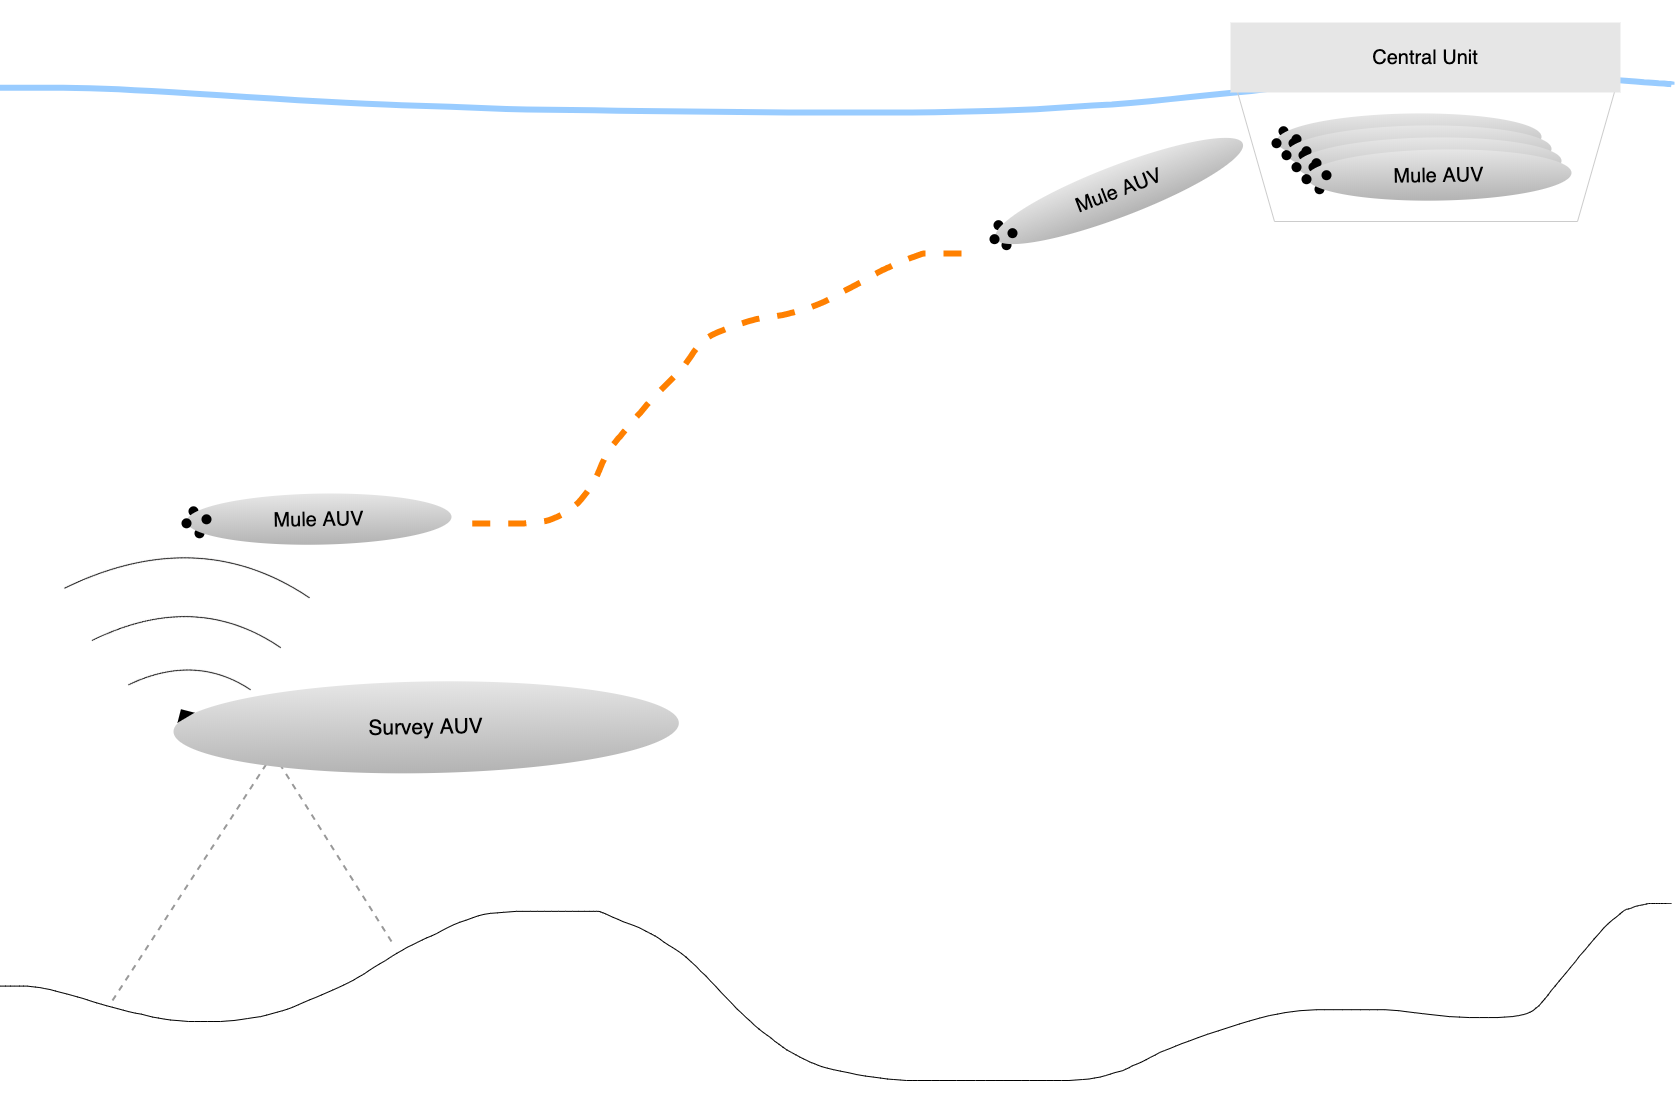
\includegraphics[width=1\textwidth]{figures/GROW}
	\caption{Illustration of the GROW project}
	\label{fig:grow}
\end{figure}

%\begin{figure}[!htbp]
%	\centering
%	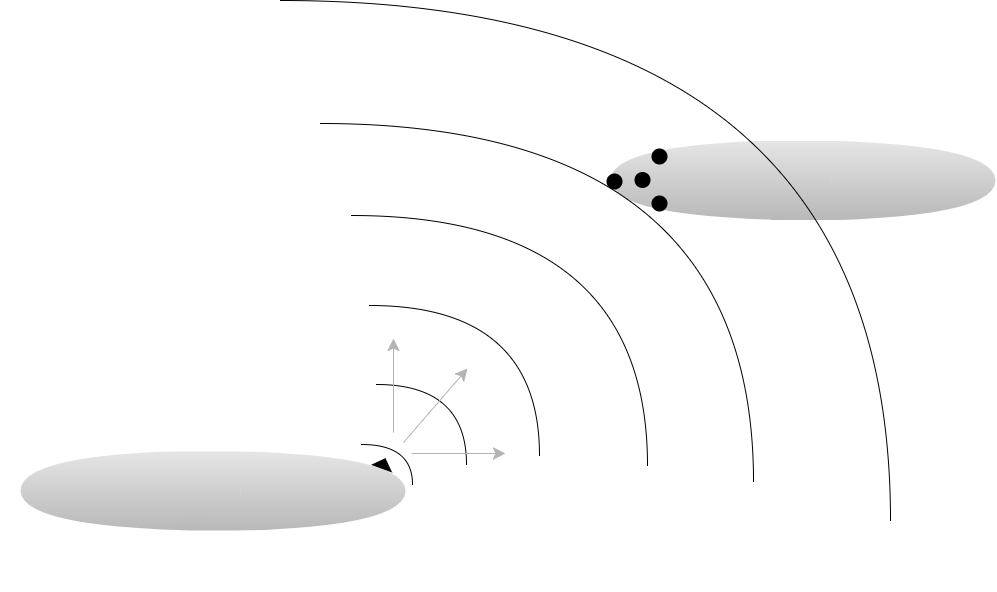
\includegraphics[width=0.8\textwidth]{figures/proposed-solution}
%	\caption{Communication System}
%	\label{fig:auv_scene}
%\end{figure}

This partial USBL system was developed in previous dissertations and research work, which can be better understood in \cite{afonso-thesis}. Briefly, the system consists on a transducer of four hydrophones forming a 3D array deployed on the mule AUV. The distance between AUVs is given by the cross-correlation between the received and expected signals. Since the operation frequency range is around tens of kilohertz, which minimizes the attenuation of sound, the time difference of arrival has to be refined by analyzing the relative phase differences between hydrophones.

Considering that the survey AUV navigates freely trough unknown locations, the USBL system to be employed needs to fulfill particular requirements that common commercial solutions do not comply. 

Firstly, the system needs to be able to cover both short and long range distances, going from tens of centimeters to several hundreds of meters between the receiver and the transmitter, with the best estimation precision possible. For long range positions, the precision of the estimation affects how direct is the path for the mule AUV to reach the acoustic source. This influences the overall energy consumption, duration of navigation search and can affect the reliability of the process. For short range position, an accurate estimate allows to avoid collisions and correctly establish chosen relative positions between vehicles. Additionally, an increase in the frequency of position estimation would consume more power but provide more robust positions, which is desirable for short range scenarios. The available market systems usually offer multiple solutions with different limited operation ranges, which would force to employ more than one system to achieve the mentioned range requirement.

Secondly, the USBL system needs to be capable of detecting incoming signals from any position in space, since the localization detection is solely based on the received signals. Since the system is composed by various sensors, it is expected that they are arranged in varied positions and with different perspectives so they can cover a wider area. However, considering they are supposed to be employed on an AUV, the vehicle's body represents an opaque obstacle to signals. Therefore, with only four fixed hydrophones, it is not possible to detect positions with full line of sight, as intended, since not all hydrophones would have line of sight to the transmitter at all times.

The system that is proposed in this dissertation intended to resolve this technological gap with a system that satisfies the described requirements. Since only four hydrophones are enough to obtain a position estimation (bearing and distance), if they assume a fixed position on an AUV's body it would inevitably limit the direction to where the sensor has direct line of sight. Therefore, the suggested method implies deploying multiple sensors in the vehicle. From the available sensors, only four would be used simultaneously to receive the signals and feed them to the processing system. By adopting this concept, a main issue that arises is where to place the hydrophones within the vehicle. This constitutes the main research topic conducted in the present thesis.

Considering that the mentioned mechanism is meant to be applied in mobile vehicles with changing environment conditions, it is useful to integrate it in a system which is responsive in real time. Accordingly, the process that selects four hydrophones among the available set can be integrated in an adaptive reconfigurable system which enables the hydrophones commutation according to the sensors' configuration that minimizes the estimation error.

The study conducted in the scope of this dissertation intends to prove the functionality of the developed method, validate the hypothesis declared in \ref{sec:hypoth-rq} and draw conclusions on the research questions.

\subsection{Assumptions} \label{sec:premises}

This research work relies on a set of premises that were considered throughout the development of the proposed system, as presented in this section.

\paragraph{Number of sensors} For the estimation of the position in 3D space, a multilateration approach was used, as explained in \ref{subsubsec:lateration}. Therefore, a minimum of 4 hydrophones are needed so that it is possible to define the position of the transmitter. Using only two sensors, two possibility spheres are formed around these sensors whose intersection originates a circle that contains the location possible solutions. By adding a third sensor, this circle is intersected by another sphere which originates only two location possibilities. Finally, a fourth sensor is added to exactly differentiate which is the accurate location solution.

\paragraph{Synchronism} The system integrates a synchronization mechanism that allows to know the time of emission of an acoustic signal, hence it is possible to compute the ToA of the signal which indicates the range between the transmitter and the receiver.

\paragraph{Noise characteristics} The system assumes an injected error $e_i$ added to the time differences of arrival, $ \Delta t_{ij}$. These errors are mutually independent and follow a Gaussian distribution with zero mean and a configurable variance of $\sigma^{2}$, i.e., $e_i \sim \mathcal{N}(0,\,\sigma^{2})$. 

For the simulations performed in this project, a deviation of 5$^{\circ}$, or a window of $[-2.5^{\circ},2.5^{\circ}]$, in phase difference estimation of incoming signals was considered to be reasonable for an underwater navigation scenario. This value is based on the observation that the process implemented to calculate the phase difference, using acoustic signals recorded in controlled laboratory environment, produced a stable value within an interval of 2 degrees. Therefore, since the specified period of the signals is $T = \frac{1}{24400}$, then the 5$^{\circ}$ will be equivalent to $\frac{5^{\circ}}{360^{\circ}}*T$ which is approximately a deviation of $0.5\mu s$. Hence the considered standard deviation $\sigma$ to characterize the error $e_i$ in the computed time differences of arrival is equal to $0.5\mu s$.

\paragraph{Reference axis} The origin of the reference axis is defined at the center of the structure where the hydrophones are fixed, which in this case is the AUV.

\paragraph{Propagation speed} The considered speed of sound is 1500 m/s, which corresponds to the underwater propagation velocity of waves in typical conditions.

%------------------------------------------------------------------------------------
\subsection{Hypothesis and Research Questions} \label{sec:hypoth-rq}

This dissertation intends to complement previous research work and answer to a core research hypothesis which serves as fundamental investigation purpose. This research hypothesis can be stated as:
\\

\textit{"Using a USBL system that reconfigures the hydrophone selection leads to an improvement on the underwater localization precision, allowing to always have a set of four active hydrophones with line of sight to the transmitter and makes it suitable for both short and long range estimation."}
\\

Attending the proposed hypothesis, there are essential topics that are intended to be explored and discussed in this thesis's work. Therefore, fours research questions were formulated which are the focus of the developed work, summarized as follows:

%Research Questions
\begin{description}
	\item[RQ1: ] \textit{What method should be adopted in order to efficiently compare the performance of hydrophone configurations?}
	
	\item[RQ2: ] \textit{What decision metric(s) should be used to evaluate the optimal hydrophone configuration for a specific angle of arrival?}
	
	\item[RQ3: ]\textit{How should the system be developed in order to assure that the selected hydrophones always have line of sight to the transmitter?}
	
	\item[RQ4: ] \textit{Are there distinct best hydrophone configurations for short and long range estimation?}
\end{description}

These questions summarize the main topic points which are explored in the scope of this thesis and are the essential inquiries that it intends to answer.

%------------------------------------------------------------------------------------
\subsection{Validation Methods} \label{sec:validation}

The validation of scientific work is a key factor to demonstrate how reliable and effective it is. In this thesis, three essential methods are used to validate the functionality of the developed techniques:

\begin{itemize}
	
	\item \textbf{Simulation}
	
	The considered immediate approach to evaluate the functionality and behavior of the system consists in creating a set of simulation procedures which are as close as possible to the real environment and the physical system. These simulations were made as MATLAB scripts carefully designed to integrate realistic parameters, such as expected environment noise and other limitations.
	
	\item \textbf{Scientifically recognized methods}
	
	When composing a system, it can be useful comparing the studied approach with widely used methods which are recognized in the scientific community. By doing this, we can gain a level of confidence in the developed system and in the obtained results.
	
	\item \textbf{Field experiments}
	
	After having the analytical methods and simulations coherent, it is essential then to test the system in a real environment in order to assess the functionality and performances when real conditions are added. By testing it in a real application it is possible to take conclusions about its robustness and consider improvements or refinements for the system.
	Due to the exceptional pandemic situation, in the present work it was only possible to perform field tests on the developed digital signal processing module. 
	
\end{itemize}


%-------------------------------------------------------------------------------------------
\section{Document Structure} \label{sec:doc-struct}

The present document is partitioned into six chapters, which are summarized in this section.

Chapter \ref{chap:sota} offers an overview on background concepts about underwater acoustics, localization estimation and positioning systems, followed by USBL available commercial solutions and developed technology for a similar purpose. Lastly, it focuses on optimization mechanisms that are typically employed for evaluating sensor configurations.

After reviewing the literature, chapter \ref{chap:hdl} explains the implemented digital signal processing module for the phase difference calculation, describing its components and design decisions. At the end, the influence of the Doppler effect is presented.

Chapter \ref{chap:proposed_sys} introduces three different approaches are presented for systematic comparison between the performance of a sensor configuration. These are supported with simulation experiments which allow to draw conclusions on the preferred approach.

Chapter \ref{chap:study} details the developed adaptive configuration selection method. The theoretical specifics and thought process are laid out and the mechanism is then validated through simulations.

Lastly, chapter \ref{chap:conclusion} gives the final remarks about the developed work, enumerates the contributions and mentions research work which could be further developed in the future.  
